\section{Medios Compartidos}
La idea es controlar el acceso a los medios compartidos de manera tal que haya la menor cantidad de intervención humana posible en el proceso. Es decir, se busca no tener la figura de un administrador que tenga que solucionar manualmente las cosas.

Tanto TDM, FDM, WDM y CDMA (Code Division Multiple Access) comparten una característica: debe estar decidido a priori qué usuario está usando qué parte del tiempo, frecuencia, etc. en cada momento. Para eso es necesario saber de antemano cuántos usuarios tendrá el sistema. Esto requiere un administrador dedicado a una red con características estáticas, rígidas.

Esto no escala de manera automática, por lo que no cumple la idea mencionada arriba. Esto no significa que estas técnicas no se usen: se utilizan frecuentemente en las redes
troncales (backbones), que no tienen una cantidad constantemente cambiante de nodos como sí puede tener algo como una red LAN, o Wi-Fi. Una alternativa a esto, para redes donde la cantidad de nodos es desconocida y cambiante, es la \textbf{contención estadística}. Esto se refiere a sistemas en los cuales varios usuarios comparten un canal común, de modo tal que puede dar lugar a conflictos conocidos como sistemas de
contención. Estos conflictos son aceptados y/o manejados.

\paragraph{Problemas de acceso:} Si hay varios nodos que usan un medio físico compartido, la simultaneidad de transmisión no es posible (no pueden transmitir todos a la vez). Para esto aparecen los \textbf{MAC Protocols (Medium Access Control)}, protocolos que buscan maximizar, en promedio, el número de éxitos en los intentos de comunicación, y asegurar la igualdad de oportunidades (en promedio) entre todos los nodos competidores.

En estos casos, el control es descentralizado, y surge la necesidad de un esquema de direccionamiento y de controlar el acceso.

Ejemplos: Aloha, Ethernet, Wi-Fi, Token Ring.

\subsection{Ethernet (IIEEE 802.3)}
Las computadoras de un edificio se conectan entre sí por medio de cables. Cada versión de Ethernet tiene un máximo de distancia física entre segmentos. Para permitir conexiones de mayor distancia se pueden utilizar \textbf{repetidores}, que son dispositivos que amplifican y retransmiten señales en ambas direcciones.
El formato utilizado para enviar mensajes en la red es el siguiente:

\begin{figure}[H]
	\centering
	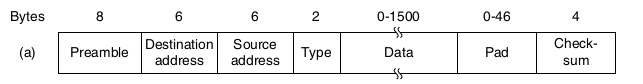
\includegraphics[width=\textwidth
]{images/ethernet-mac-frame.png}
	\caption[Frame del protocolo Ethernet]{Frame del protocolo Ethernet}
	\label{fig:ethernet-mac-frame}
\end{figure}

\begin{itemize}
  \item Los primeros 8 bytes son un preambulo que permiten a los receptors sincronizarse con la señal.
  \item Luego, vienen dos direcciones, cada uno de 6 bytes. 
  
  Cuando el primer bit de la dirección de destino es un 0, significa que el paquete está dirigido a una máquina específica.  Si es un 1, entonces es un dirección grupal: Estas direcciones permiten que varias máquinas escuchen una única dirección y que todas las máquinas pertenecientes al grupo reciban los paquetes dirigidas a esa dirección. Este tipo de envío se llama \textbf{multicasting}. Además, la dirección especial que consiste en todos bits de valor 1 está reservada para hacer \textbf{Broadcasting} (enviar un mensaje a todos los dispositivos de la red).
  \item Los próximos 2 bytes identifican el tipo de protocolo que debe usarse para procesar el contenido del paquete.
  \item Después viene la información per se que puede ocupar hasta 1500 bytes (un valor decidido de manera arbitraria).
  \item Si la data enviada es menor a 46 bytes, se usa padding hasta completar los 46 bytes necesarios para cumplir con los requirimientos de longitud mínima del mensaje. Esta longitud mínima permite que la máquina de origen detecte colisiones durante la transmición, en el caso de haberlas (más adelante explicado).
  \item Los últimos 4 bytes del paquete son un checksum (CRC de 32 bits) que permite detectar si hubo algún error en el frame, si lo hubo, el frame se descarta.
\end{itemize}

\subsubsection{Colisiones}
Una de las razones para tener una longitud mínima de un frame es para evitar que una máquina termine de transmitir el frame antes de que el primer bit haya alcanzado el otro extremo del cable, donde podría colisionar con otro frame.

\begin{figure}[H]
	\centering
	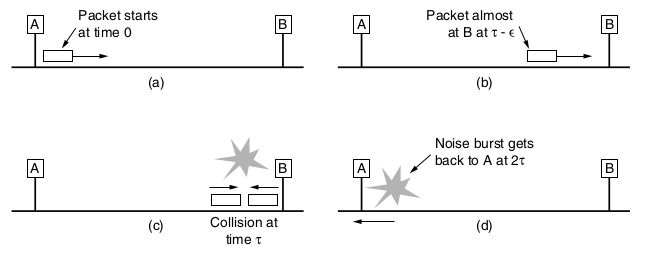
\includegraphics[width=\textwidth
]{images/deteccion-colisiones.png}
	\caption[Detección de Colisiones]{Detección de Colisiones}
	\label{fig:deteccion-colisiones}
\end{figure}

Supongamos que en un timpo 0, el host \(A\) comienza a transmitir el paquete. Sea   \(\tau\) el tiempo de propagación necesario para que el frame llegue al host \(B\). Supongamos que justo antes de que el frame llegue a destino, en el tiempo \(\tau-\epsilon\), \(B\) comienza a transmitir. Cuando \(B\) detecta que está recibiendo más energía que la que está emitiendo, se da cuenta que ocurre una colisión, aborta su propia transmisión y genera una rafaga de sonido ee 48 bits para alertar a las demás estaciones. 

En otras palabras, genera interferencia para asegurarse que el emisor (\(A\)) se de cuenta de que ocurrió la colisión. En el momento \(2\tau\), \(A\) ve el sonido y aborta su propia transmición. Luego espera un intervalo de tiempo random antes de intentar de nuevo.

Si \(A\) trata de enviar un frame muy corto, puede llegar a pasar que termine de trasmitir antes de que  perciba el ruido generado por \(B\) (en el momento \(2\tau\)). Entonces \(A\) concluiria que el frame se envió correctamente. Por esta razón, se utiliza el pading en el frame de Ethernet para completar la longitud mínima de 64 bytes.

Este valor se deduce de las especificacioens de IIEEE 802.3: Para una red de 10Mbps con una longitud de 2500 metros y a lo sumo 4 repetidores, se determinó que el round-trip time es de 50 \(\mu\)segundos, asi que 500 bits es el frame más corto posible para detectar colisiones. Este valor se redondeó a 512 bits (64 bytes).

\subsubsection{CSMA/CD con Exponential BackOff}\label{section::csma}
CSMA/CD (Carrier Sense Multiple Access with Collision Detection), es decir, acceso múltiple con sensado de portadora y detección de colisiones, es un algoritmo de control de acceso a un medio compartido.

Utiliza el sensado de portadora para determinar si hay nodos transmitiendo. Cuando un host tiene datos para enviar, sensa el medio compartido:
\begin{itemize}
  \item Si el medio está libre, el host transmite.
  \item Si el medio está ocupado, no puede enviar porque habría una colisión. Entonces debe esperar a que el medio se libere:
  \begin{itemize}
    \item Si el algoritmo es \textbf{1-persistente}, el host comienza a transmitir apenas se libere el medio.
    \item Si es \textbf{p-persistente}, el host espera a que se libere el medio y transmite con probabilidad \(p\). El uso de un componente azaroso (en la p-persistencia) tiene sentido porque si hay varios
    hosts esperando a que se libere el medio, y todos intentan transmitir ni bien éste se libera, va
    a ocurrir una colisión. Imponer una probabilidad para transmitir reduce las probabilidades de
    colisiones.
  \end{itemize}
\end{itemize}

Este algoritmo es de categoría half-duplex: La lógica de recepción está establecida en el sensado para detectar colisiones. Es decir, no se puede enviar y recibir a la vez (eso sería full-duplex).

Supongamos ahora que ocurre una colisión, entonces el tiempo se divide en slots de tamaño \(2\tau\). Después de la primera colisión, cada estación espera 0 o 1 slots de tiempo al azar. Si dos estaciones colisionan y eligen el mismo número, cada una elige entre 0, 1, 2 ó 3 tiempos al azar y espera el número de slots de tiempos elegidos antes de volver a intentar transmitir.

En general, después de la \(i\)-ésima colisión, cada host debe elegir un número entre 0 y \(2^i-1\) que será la cantidad de slots de tiempo que debe dejar pasar antes de volver a intentar la transmición.

Este algoritmo se llama \textbf{Exponential Backoff Binario}, sirve para adaptar de manera dinámica el número de estaciones que están tratando de emitir simultaneamente. Si el intervalo de elección para todas las elecciones fuese 1023, las chances de colisión son despreciables.


\begin{figure}[H]
	\centering
	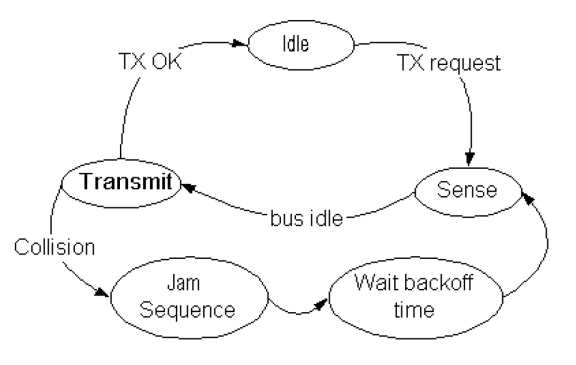
\includegraphics[width=\textwidth
]{images/csma-cd.png}
	\caption[Topologías de Red]{Topologías de Red}
	\label{fig:csma-cd}
\end{figure}

\subsubsection{Logical Link Control}
Es la subcapa de la capa de enlace que se encarga de procesar el paquete recibido en la capa MAC y enviarlo al proceso correspondiente en la capa de Red.

\subsection{Redes inalámbricas: Wi-Fi: IEEE 802.11b/g/n}
En las redes inalámbricas, los frames se mandan a través de ondas en una determinada frecuencia, que depende de la tecnología usada para transmitirlas. En este tipo de red, la intensidad de la señal disminuye con la distancia y tiene fuentes de ruidos más impredecibles que en medios guiados. Esto se traduce en una tasa de errores elevadas.

\subsubsection*{Spread Spectrum}
Esto sumado a que cualquier dispositivo cercarno puede conectarse a ellas, impulsaron el diseño de técnicas para aprovechar al máximo el ancho de banda de tal forma de proteger a la red de intrusos. Est técnica es llamada \textbf{Spread Spectrum}.

Esta técnica modula la señal usando una moduladora semi random compuesta de 1s y -1s conocida por los dispositivos de la red qur aplican a la señal que quieren enviar. Cuando la señal llega el receptor, este realiza el proceso inverso para conseguir la señal original.

Otra forma de realizar esto, es enviar la información transmitida en un rango de frecuencias que es cambiado varías veces durante el proceso de transmición. En este método, la información original se divide en partes más pequeñas usando un patron conocido solamente por el transmisor y el receptor.

\subsubsection{Carrier Sense Multiple Access / Collision Avoidance (CSMA/CA)}

Dado que las redes inalámbricas son un medio de broadcasting, los equipos de la red debe estar atentos a multiples transmiciones realizadas simultaneamente. 
A diferencia de los medios guiados, implementar una comunicación full-duplex sobre radio frecuencias es costoso por lo que se intenta evitar las colisiones en vez de resolverlas.

Para manejar esto, se utiliza el sistema CSMA descripto en la sección \ref{section::csma} pero adaptado a los problemas introducidosra minimizar la probabilidad de colisiones. Si durante este período, el medio se libera, el host puede transmitir una nueva trama. Si no, se vuelve a esperar un nuevo período de contentción. por el nuevo medio que es mucho más lento:

\subsubsection*{Colission Avoidance}
Antes de transmitir, una estación debe determinar el estado del medio. Si el canal no está ocupado, se realiza una espera adicional llamada \textbf{espaciado entre tramas} para asegurarnos de que no colisione.  Si durante esta espera, el medio no permanece libre, entonces se suspende la transmición hasta que se cumpla dicha condición.

Cuando la trama se transmitió, se espera recibir un ACK. Si esto no sucede, se asume que se perdió en una colisión y se retransmitirá la misma. 

Una vez que un host transmite una trama exitosamente, espera un \textbf{período de contención} (cuantificado por un back-off) para minimizar la probabilidad de colisiones. Si durante este período, el medio se libera, el host puede transmitir una nueva trama. Si no, se vuelve a esperar un nuevo período de contención.

Este método recién descripto es llamado \textbf{Distributed Coordination Function (DCF)} y es el método de acceso al medio más básico de 802.11.


\begin{figure}[H]
	\centering
	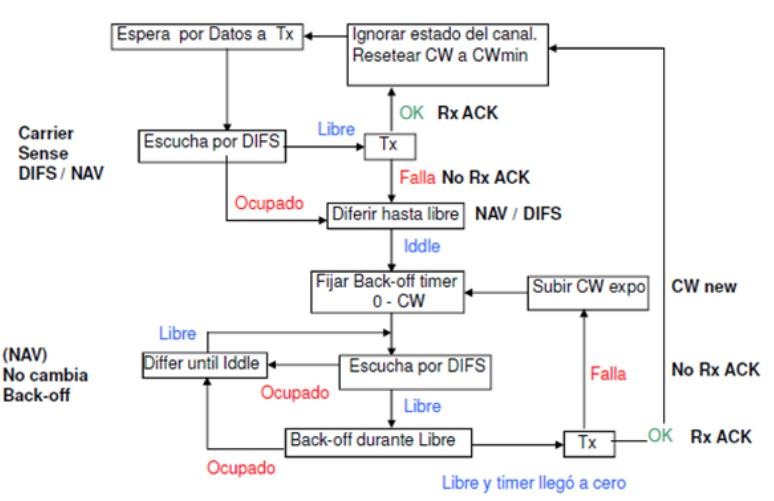
\includegraphics[width=\textwidth
]{images/wifi-estados.jpg}
	\caption[Máquina de estados de un host en una red Wifi]{Máquina de estados de un host en una red Wifi}
	\label{fig:wifi-estados}
\end{figure}

\subsubsection*{Problema de la estación oculta}
Supongamos que la computadora \(A\) comienza a transmitir a \(B\). 

Si \(C\) detecta el medio no escuchará a \(A\) porque está fuera de su alcance, y por lo tanto deducirá erroneamente que puede transmitir. Si lo hace, interferirá en \(B\) eliminando la trama de \(A\).

\begin{figure}[H]
	\centering
	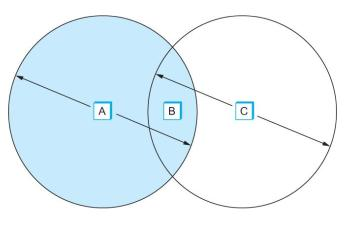
\includegraphics[width=0.5\textwidth
]{images/estacion-oculta.jpg}
	\caption[Problema de la estación oculta]{Problema de la estación oculta}
	\label{fig:estacion-oculta}
\end{figure}

\subsubsection*{Problema de la estación expuesta}
\begin{figure}[H]
	\centering
	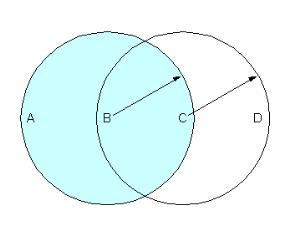
\includegraphics[width=0.5\textwidth
]{images/estacion-descubierta.jpg}
	\caption[Problema de la estación expuesta]{Problema de la estación expuesta}
	\label{fig:estacion-expuesta}
\end{figure}

Supongamos ahora que \(A\) está transmitiendo una tramba a \(B\). Supongamos ahora que \(C\) quiere transmitir a \(D\), cuando detecta al medio, escuhará una transmición y concluirá que no puede realizar su envio. Sin embargo, esa transmición causaría una mala recepción solo en la zona entre \(B\) y \(C\), en la que no está localizado ninguno de los receptores pretendidos.
